%%%%%%%%%%%%%%%%%%%%%%%%%%%%%%%%%%%%%%%%%
% Stylish Article
% LaTeX Template
% Version 2.1 (1/10/15)
%
% This template has been downloaded from:
% http://www.LaTeXTemplates.com
%
% Original author:
% Mathias Legrand (legrand.mathias@gmail.com) 
% With extensive modifications by:
% Vel (vel@latextemplates.com)
%
% Authors:
% Mauricio Hoyos Ardila mhoyosa2@eafit.edu.co
% Jonathan Zapata Castaño jzapat80@eafit.edu.co
%
% License:
% CC BY-NC-SA 3.0 (http://creativecommons.org/licenses/by-nc-sa/3.0/)
%
%%%%%%%%%%%%%%%%%%%%%%%%%%%%%%%%%%%%%%%%%

%----------------------------------------------------------------------------------------
%	PACKAGES AND OTHER DOCUMENT CONFIGURATIONS
%----------------------------------------------------------------------------------------

\documentclass[fleqn,10pt]{SelfArx} % Document font size and equations flushed left

\usepackage[english]{babel} % Specify a different language here - english by default

\usepackage{lipsum} % Required to insert dummy text. To be removed otherwise

%----------------------------------------------------------------------------------------
%	COLUMNS
%----------------------------------------------------------------------------------------

\setlength{\columnsep}{0.55cm} % Distance between the two columns of text
\setlength{\fboxrule}{0.75pt} % Width of the border around the abstract

%----------------------------------------------------------------------------------------
%	COLORS
%----------------------------------------------------------------------------------------

\definecolor{color1}{RGB}{0,0,0} % Color of the article title and sections
\definecolor{color2}{RGB}{0,20,20} % Color of the boxes behind the abstract and headings

%----------------------------------------------------------------------------------------
%	HYPERLINKS
%----------------------------------------------------------------------------------------

\usepackage{hyperref} % Required for hyperlinks
\hypersetup{hidelinks,colorlinks,breaklinks=true,urlcolor=color2,citecolor=color1,linkcolor=color1,bookmarksopen=false,pdftitle={Title},pdfauthor={Author}}

%----------------------------------------------------------------------------------------
%	ARTICLE INFORMATION
%----------------------------------------------------------------------------------------

\JournalInfo{Reporte Técnico, No. 1, 2017} % Journal information
\Archive{Universidad EAFIT} % Additional notes (e.g. copyright, DOI, review/research article)

\PaperTitle{Agrupamiento de Documentos usando K-means} % Article title

\Authors{Mauricio Hoyos\textsuperscript{1}, Jonathan Zapata\textsuperscript{2}} % Authors
\affiliation{\textsuperscript{1}\textit{Departamento de Ingeniería de Sistemas, Universidad EAFIT, Medellín, Colombia, } \textbf{mhoyosa2@eafit.edu.co}} % Author affiliation
\affiliation{\textsuperscript{2}\textit{Departamento de Ingeniería de Sistemas, Universidad EAFIT, Medellín, Colombia, } \textbf{jzapat80@eafit.edu.co}} % Author affiliation

\Keywords{K-means --- Jacard --- MPI --- Cluster --- HPC } % Keywords 

\newcommand{\keywordname}{Keywords} % Defines the keywords heading name

%----------------------------------------------------------------------------------------
%	ABSTRACT
%----------------------------------------------------------------------------------------

\Abstract{Text mining is an analysis technique which has allowed us to implement a set of new applications at the day. Such as search engines in the web (Google, Facebook, Amazon, Spotify, Netflix, among others), suggestions systems, natural language processing.
The document clustering techniques enable us to link a document with other similar documents according to a comparison metric.}

%----------------------------------------------------------------------------------------

\begin{document}

\flushbottom % Makes all text pages the same height

\maketitle % Print the title and abstract box

\tableofcontents % Print the contents section

\thispagestyle{empty} % Removes page numbering from the first page

%----------------------------------------------------------------------------------------
%	ARTICLE CONTENTS
%----------------------------------------------------------------------------------------

\section*{Introducción} % The \section*{} command stops section numbering

\addcontentsline{toc}{section}{Introducción} % Adds this section to the table of contents

Actualmente, debido a la gran cantidad de información que se encuentra en los medios, surge la necesidad de agrupar dicha información en un conjunto de datos que permita realizar búsquedas más rápidas, para ello se  crearon técnicas que permiten calcular la similitud que tienen dos textos, una de las más utilizadas es la minería de datos, la cual, como su nombre lo indica, se encarga de extraer las partes importantes de un archivo (en nuestro caso un texto), el enfoque que le dimos al proyecto está delimitado precisamente por esta área de la ciencia de datos, la cual nos va a permitir crear varios set de documentos y determinar el número de sets apropiados que deberíamos generar.
La técnica de agrupamiento de documentos 

 and some mathematics $\cos\pi=-1$ and $\alpha$ in the text\footnote{And some mathematics $\cos\pi=-1$ and $\alpha$ in the text.}.

%------------------------------------------------

\section{Marco Teórico}

\subsection{Descripción del Problema}
\begin{figure*}[ht]\centering % Using \begin{figure*} makes the figure take up the entire width of the page
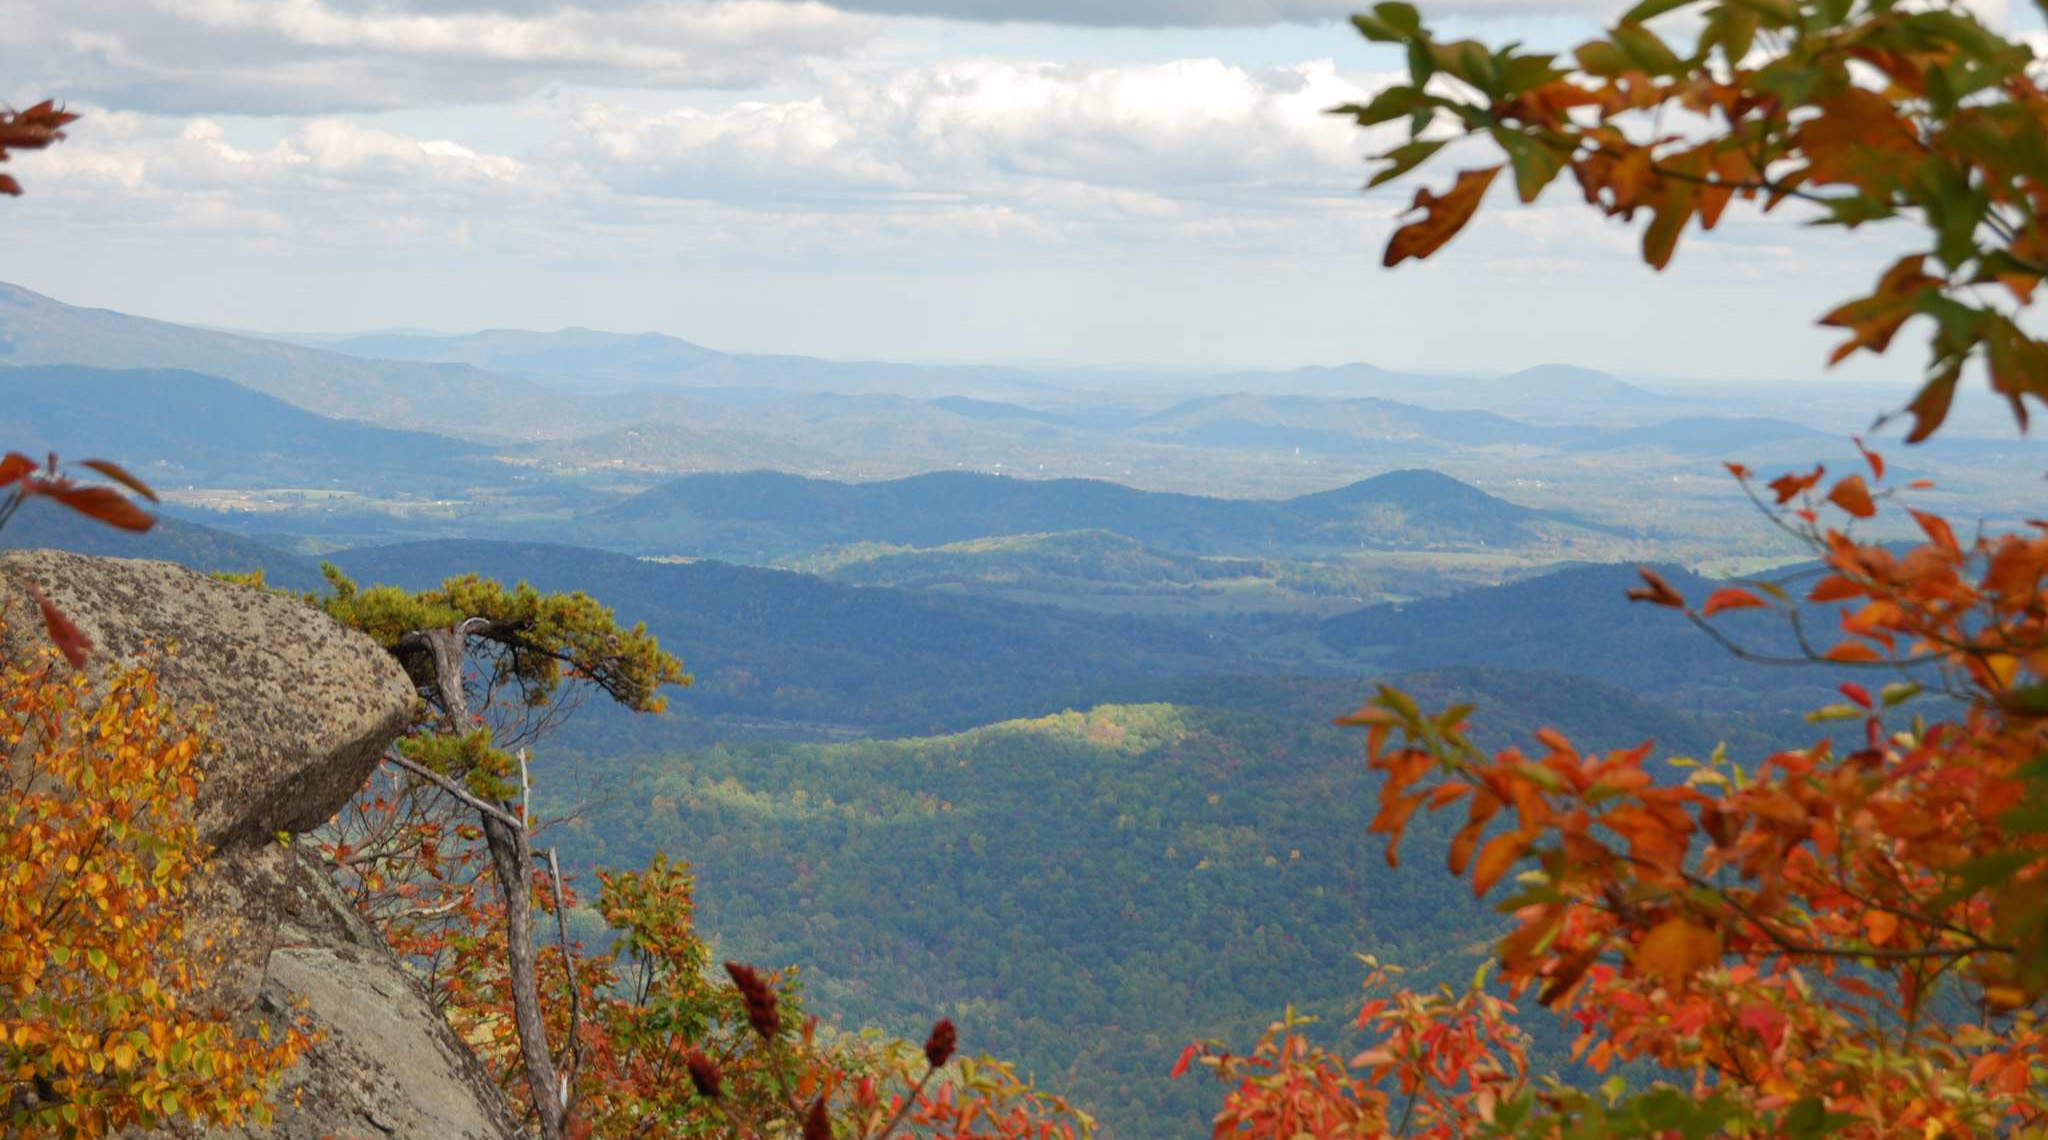
\includegraphics[width=\linewidth]{view}
\caption{Wide Picture}
\label{fig:view}
\end{figure*}

\lipsum[4] % Dummy text

\begin{equation}
\cos^3 \theta =\frac{1}{4}\cos\theta+\frac{3}{4}\cos 3\theta
\label{eq:refname2}
\end{equation}

\lipsum[5] % Dummy text

\begin{enumerate}[noitemsep] % [noitemsep] removes whitespace between the items for a compact look
\item First item in a list
\item Second item in a list
\item Third item in a list
\end{enumerate}

\subsection{Subsection}

\lipsum[6] % Dummy text

\paragraph{Paragraph} \lipsum[7] % Dummy text
\paragraph{Paragraph} \lipsum[8] % Dummy text

\subsection{Subsection}

\lipsum[9] % Dummy text

\begin{figure}[ht]\centering
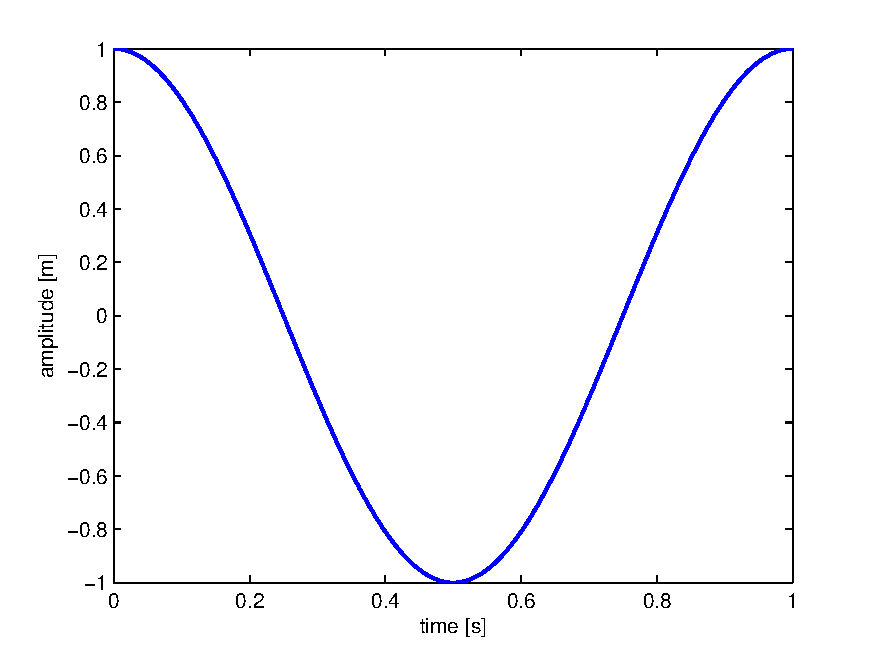
\includegraphics[width=\linewidth]{results}
\caption{In-text Picture}
\label{fig:results}
\end{figure}

Reference to Figure \ref{fig:results}.

%------------------------------------------------

\section{Análisis y Diseño (PCAM)}

\lipsum[10] % Dummy text

\subsection{Subsection}

\lipsum[11] % Dummy text

\begin{table}[hbt]
\caption{Table of Grades}
\centering
\begin{tabular}{llr}
\toprule
\multicolumn{2}{c}{Name} \\
\cmidrule(r){1-2}
First name & Last Name & Grade \\
\midrule
John & Doe & $7.5$ \\
Richard & Miles & $2$ \\
\bottomrule
\end{tabular}
\label{tab:label}
\end{table}

\subsubsection{Subsubsection}

\lipsum[12] % Dummy text

\begin{description}
\item[Word] Definition
\item[Concept] Explanation
\item[Idea] Text
\end{description}

\subsubsection{Subsubsection}

\lipsum[13] % Dummy text

\begin{itemize}[noitemsep] % [noitemsep] removes whitespace between the items for a compact look
\item First item in a list
\item Second item in a list
\item Third item in a list
\end{itemize}

\subsubsection{Subsubsection}

\lipsum[14] % Dummy text

\subsection{Subsection}

\lipsum[15-23] % Dummy text

%------------------------------------------------
\phantomsection
\section*{Acknowledgments} % The \section*{} command stops section numbering

\addcontentsline{toc}{section}{Acknowledgments} % Adds this section to the table of contents

So long and thanks for all the fish \cite{Figueredo:2009dg}.

%----------------------------------------------------------------------------------------
%	REFERENCE LIST
%----------------------------------------------------------------------------------------
\phantomsection
\bibliographystyle{unsrt}
\bibliography{sample}

%----------------------------------------------------------------------------------------

\end{document}